\documentclass[a4paper,11pt,oneside]{book}
\usepackage[T1]{fontenc}                                      
\usepackage[utf8]{inputenc}                               
\usepackage[italian]{babel}
\usepackage{titlesec, blindtext, color}
\usepackage{graphicx}
\usepackage{amsmath,amssymb}
\usepackage{textcomp}
\usepackage{makeidx}
\usepackage{epsfig}
\usepackage{mathrsfs}


\begin{document}
\setcounter{chapter}{9}
\chapter{Problemi Unidimensionali}
\section{Proprietà generali dell'equazione di Schr\"{o}dinger}
La funzione d'onda deve essere monotona e continua in tutto lo spazio.\\
le derivate della f.d.o. sono continue ovunque, anche su superfici di discontinuità del potenziale, eccetto il caso in cui $V$ diventa infinito al di fuori di tali superfici.\\
Una particella non può penetrare un generale in una regione dello spazio dove $V =\infty$, cioè dappertutto in questa regione la f.d.o. è nulla. La continuità delle f.d.o. esige che essa si annulli sul contorno di questa regione, quanto alle derivate della f.d.o. esse subiscono allora, in generale, un salto.\\
Se il potenziale $V$ è ovunque finito, anche la f.d.o. deve essere finita in tutto lo spazio (questa condizione deve essere ugualmente soddisfatta nei casi in cui $V$ diventa infinito in un punto ma non non troppo rapidamente: come $1/r^s$ con $s<2$).\\
Tutti gli autovalori dell'energia sono maggiori del minimo valore assoluto del potenziale $V$, cioè:
\begin{equation}
E_n >V_{min} \quad \forall n.
\end{equation}
Allo stesso tempo, una particella in Meccanica Quantistica può venire anche a trovarsi nelle regioni dello spazio in cui $E<V$. Anche se la probabilità $|\psi|^2$ di presenza della particella tende rapidamente a zero all'interno di tale regione, essa è però differente da zero a tutte le distanze finite.\\ \\
È semplice dimostrare che gli autovalori dell'energia sono sempre maggiori del minimo del potenziale. Si ha infatti:
\begin{equation}
E_n = \langle n | H |n \rangle = \langle n | \frac{p^2}{2m} |n \rangle + \langle n | V(x) |n \rangle.
\end{equation}
I due valori medi soddisfano poi:
\begin{equation}
\langle n | \frac{p^2}{2m} |n \rangle \geq 0,
\end{equation}
\begin{equation}
\langle n | V(x) |n \rangle = \int _{-\infty} ^{+\infty} dx' V(x')|\psi _n(x')|^2 \geq V_{min} \int _{-\infty} ^{+\infty} dx' |\psi _n(x')|^2 = V_{min},
\end{equation}
da cui segue:
\begin{equation}
E_n \geq V_{min} \qquad \textrm{c.v.d.}
\end{equation}
\section{Particella su un segmento (buca di potenziale infinita)}
Consideriamo una particella nel campo di potenziale:\\

\begin{minipage}{.5\textwidth}
\begin{align}
V(x)= 
\begin{cases}
\infty \quad x<0,\\
0 \quad 0>x>a, \\
\infty \quad x>a.
\end{cases}
\\
\textrm{(buca di potenziale infinita)} \nonumber
\end{align}	
\end{minipage}
\hspace{.5cm}
\begin{minipage}{.4\textwidth}
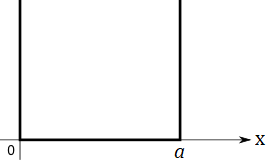
\includegraphics[width=\textwidth]{immagini/cap_10/fig_10_1.png}
\end{minipage}\\


Il moto della particella può avvenire soltanto nel segmento $\left( 0; a \right)$, giacché non è posisbile che questa penetri che questa penetri in una regione in cui $V=\infty$. Allora:
\begin{equation}
\psi(x)= 
\begin{cases}
0\quad x<0,\\
0 \quad x>a.
\end{cases}
\end{equation}
All'interno della buca, dove $V(x)=0$, l'eq. di Schr\"{o}dinger ha la forma:
\begin{equation}
-\frac{\hbar ^2}{2m}\frac{d^2 \psi}{dx^2}= E\psi\quad \Longrightarrow \quad \frac{d^2 \psi}{dx^2}=-\frac{2mE}{\hbar^2}\psi,
\end{equation}
che deve essere risolta con le condizioni al contorno:
\begin{equation}
\psi(0)=\psi(a)=0,
\end{equation}
richieste dalla continuità della f.d.o. in $x=0$ e $x=a$.\\
È facile verificare che \textbf{l'equazione non ha soluzioni corrispondenti ad $\textbf{E=0}$}, in accordo con la proprietà generale secondo cui gli autovalori dell'energia sono sempre maggiori del minimo del potenziale, in questo caso $V_{min}=0$. Infatti, per $E<0$ si può porre:
\begin{equation}
\lambda ^2 = -\frac{2mE}{\hbar ^2},
\end{equation}
e l'equazione di Schr\"{o}dinger diventa:
\begin{equation}
\frac{d^2 \psi}{dx^2}=\lambda ^2\psi.
\end{equation}
Le soluzioni di questa equazione sono della forma:
\begin{equation}
\psi(x)= Ae^{\lambda x}+ Be^{-\lambda x}.
\end{equation}
la condizione in $\psi (0)=0$ implica:
\begin{equation}
\psi(0)= A+ B=0 \quad \Rightarrow \quad B=-A,
\end{equation}
ossia
\begin{equation}
\psi(x)= 2A \sinh{\left( \lambda x \right)},
\end{equation}
e la condizione $\psi(a)=0$ non risulta mai soddisfatta.\\
Considerando allora $\textbf{E>0}$ e ponendo
\begin{equation}
k ^2 = \frac{2mE}{\hbar ^2},
\end{equation}
otteniamo per l'equazione di Schr\"{o}dinger l'espressione:
\begin{equation}
\frac{d^2 \psi}{dx^2}=-k ^2\psi.
\end{equation}
La soluzione generale di questa equazione è
\begin{equation}
\psi(x)= Ae^{ik x}+ Be^{-ik x}.
\end{equation}
la condizione $\psi (0)=0$ richiede:
\begin{equation}
\psi(0)= A+ B=0 \quad \Rightarrow \quad B=-A,
\end{equation}
ossia
\begin{equation}
\psi(x)= 2iA \sin{\left( k x \right)},
\end{equation}
la condizione in $\psi (a)=0$ implica:
\begin{equation}
k_n a= n\pi \qquad n=1,2,3\dots
\end{equation}
Questa è la condizione che determina gli \textbf{autovalori discreti dell'energia}:
\begin{equation}
E_n= \frac{\hbar ^2 {k_n}^2}{2m}=\frac{\hbar ^2 \pi n^2}{2ma^2} \quad n=1,2,3,\dots
\end{equation}
Le corrispondenti autofunzioni sono:
\begin{equation}
\psi _n = 2iA_n \sin{\left( k_n x\right)} \Rightarrow 2A_n \sin{\left( k_n x \right)},
\end{equation}
dove abbiamo tolto il fattore di fase irrilevante $i$.\\
La costante complessa $A_n$ può essere determinata dalla \textbf{condizione di normalizzazione}:
\begin{equation}
\int _{-\infty} ^{\infty} |\psi(x)| ^2 dx =1.
\end{equation}
Si trova:
\begin{eqnarray}
\int _{-\infty} ^{\infty} |\psi(x)| ^2 dx &=& \int _{0} ^{a} 4|A_n| ^2 \sin ^2 {\left( k_n x \right)}\ dx= \nonumber \\
&=& 4|A_n| ^2 \int _{0} ^{a} \left( \frac{e^{ik_n x}- e^{-ik_nx}}{2i}\right) ^2\ dx = \nonumber \\ 
&=& -|A_n| ^2 \int _{0} ^{a} \left( e^{2ik_n x}+ e^{-2ik_nx}-2\right)\  dx = \nonumber \\
&=& |A_n| ^2 \left[ 2a- 2 \int _{0} ^{a} \cos \left(\frac{2n \pi}{a} x\right)\   dx \right] = \nonumber \\
&=& |A_n| ^2 \left[ 2a- \frac{a}{n\pi} \int _{0} ^{2n\pi} \cos \alpha\   d\alpha \right] = \nonumber \\
&=& 2a|A_n|^2= 1.
\end{eqnarray}
Scegliendo la fase arbitraria della f.d.o. in modo tale che $A_n$ risulti reale e positivo otteniamo:
\begin{equation}
A_n = \frac{1}{\sqrt{2a}},
\end{equation}
ossia, in definitiva:
\begin{equation}
\psi _n (x)= \sqrt{\frac{2}{a}} \sin{\left( k_n x\right)} = \sqrt{\frac{2}{a}} \sin{\left( \frac{n \pi x}{a}\right)}; \qquad 0<x<a.
\end{equation}
È semplice verificare che \textbf{le autofunzioni sono ortogonali tra loro}:
\begin{equation}
\int _{-\infty} ^{\infty} dx\ \psi_n ^* (x) \psi _m (x) = \delta _{mn},
\end{equation}
come previsto in generale per le autofunzioni di un operatore hamiltoniano.\\ \\
\textbf{Una qualunque f.d.o.} $\mathbf{\psi (x)}$\textbf{, soluzione dell'equazione di Schr\"{o}dinger può essere espressa come combinazione lineare delle autofunzioni della hamiltoniana}:
\begin{equation}
\psi (x) = \sum _{n=1} ^{\infty} c_n \psi _n (x) = \sum _{n=1} ^{\infty} c_n \sqrt{\frac{2}{a}} \sin {\left( k_n x \right)}.
\end{equation}
L'ortonormalità delle autofunzioni può essere utilizzata per esprimere \textbf{i coefficienti} $\mathbf{c_n}$ \textbf{dello sviluppo come}:
\begin{equation}
c_n = \int _{-\infty} ^{+\infty} dx\ \psi _n ^* (x) \psi(x).
\end{equation}
Si ha infatti:
\begin{equation}
\int _{-\infty} ^{+\infty} dx\ \psi _n ^* (x) \psi(x)= \sum _m c_m \int _{-\infty} ^{+\infty} dx\ \psi _n ^* (x) \psi _m(x)= c_n.
\end{equation}
I moduli quadri $|c_n|^2$ rappresentano la probabilità che una misura dell'energia fornisca come risultato il valore $E=E_n$.\\
Il valore medio dell'energia nello stato descritto dalla f.d.o. $\psi$ è:
\begin{eqnarray}
\langle H \rangle &=& \int _{-\infty} ^{+\infty} dx\ \psi ^*(x) H \psi(x) =\sum _n c_n \int _{-\infty} ^{+\infty} dx\ \psi ^*(x) H \psi _n(x) = \nonumber \\
&=& \sum _n c_n E_n \int _{-\infty} ^{+\infty} dx\ \psi ^*(x) \psi _n(x) =\sum _n |c_n|^2 E_n .
\end{eqnarray}
Se $\psi (x)$ rappresenta la f-d-o- della particella al tempo $t=0$, la f.d.o. ad un tempo $t$ successivo è data da:
\begin{equation}
\psi (x,t) =\sum _n c_n\ e^{-\frac{i}{\hbar}E_n t}\ \psi _n (x).
\end{equation}
I risultati ottenuti consentono di derivare semplicemente gli autovalori dell'energia e le autofunzioni per una \textbf{particella in una scatola}, ossia in una buca di potenziale tridimensionale descritta dal campo:
\begin{equation}
V(x,y,z)= 
\begin{cases}
0 \quad \textrm{per}\ 0\leq x \leq a,\ 0\leq y \leq b,\ 0 \leq z \leq c;\\
\infty \quad \textrm{fuori.}
\end{cases}
\end{equation}
l'equazione di Schr\"{o}dinger per la particella all'interno della buca di potenziale si scrive:
\begin{equation}
-\frac{\hbar ^2}{2m} \left( \frac{\partial ^2 \psi}{\partial x^2}+\frac{\partial ^2 \psi}{\partial y^2}+\frac{\partial ^2 \psi}{\partial z^2}\right) = E \psi.
\end{equation}
La \textbf{hamiltoniana} si separa nella somma di tre termini, ciascuno dei quali è la  hamiltoniana di una particella libera unidimensionale:
\begin{equation}
H= H_x+H_y+H_z \qquad H_x= -\frac{\hbar ^2}{2m}  \frac{\partial ^2 \psi}{\partial x^2}, \dots
\end{equation}
Le \textbf{autofunzioni} si scompongono nel prodotto di tre autofunzioni per la buca di potenziale unidimensionale:
\begin{eqnarray}
\psi _{n_x n_y n_z} (x,y,z) &=& \psi _{n_x}(x)\psi _{n_y}(y)\psi _{n_z}(z)= \nonumber \\
&=&\sqrt{\frac{8}{abc}}\sin \frac{\pi n_x x}{a}\ \sin \frac{\pi n_y y}{b}\ \sin \frac{\pi n_z z}{c}.
\end{eqnarray}
Gli \textbf{autovalori} dell'energia sono dati dalla somma dei corrispondenti autovalori del caso unidimensionale. Scrivendo esplicitamente l'equazione agli autovalori si trova infatti:
\begin{eqnarray}
H\psi  &=& \left(H_x+H_y+H_z\right) \psi _{n_x}(x)\psi _{n_y}(y)\psi _{n_z}(z)= \nonumber \\
&=& \left( E_{n_x}+E_{n_y}+E_{n_z}\right) \psi _{n_x}(x)\psi _{n_y}(y)\psi _{n_z}(z)=  E\psi,
\end{eqnarray}
ossia, esplicitamente:
\begin{equation}
E_{n_x n_y n_z}=\frac{\hbar ^2 \pi^2}{2m} \left(\frac{{n_x}^2}{a^2}+\frac{{n_y}^2}{b^2}+\frac{{n_z}^2}{c^2}\right) \qquad n_x, n_y, n_z, = 1,2,3... 
\end{equation}
\section{Buca di potenziale: stati legati}
Consideriamo il moto di una particella nel campo di potenziale:\\

\begin{minipage}{.55\textwidth}
\begin{align}
\begin{cases}
V(x)=-V_0 \quad -a< x < a;\\
V(x)= 0 \quad x<-a,\ x> a.
\end{cases}
\\
\textrm{(buca di potenziale finita)} \nonumber
\end{align}	
\end{minipage}
\hspace{.2cm}
\begin{minipage}{.4\textwidth}
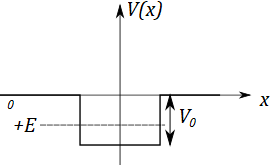
\includegraphics[width=5cm]{immagini/cap_10/fig_10_2.png}
\end{minipage}\\


Discutiamo in particolare le soluzioni dell'equazione di Schr\"{o}dinger corrispondenti agli \textbf{stati legati} della particella, ossia a valori negativi dell'energia, $\mathbf{E<0}$.\\
nelle regioni in cui il potenziale è rispettivamente nullo o pari a $-V_0$ l'equazione di Schr\"{o}dinger si scrive:
\begin{equation}
\begin{cases}
\displaystyle{-\frac{\hbar ^2}{2m}\frac{d^2 \psi}{d x^2}=-|E| \psi \qquad  x<-a,\ x> a;}\\
\\
\displaystyle{-\frac{\hbar ^2}{2m}\frac{d^2 \psi}{d x^2}= \left( V_0-|E| \right)\psi \quad  -a< x < a.}
\end{cases} 
\end{equation}
Ponendo:
\begin{equation}
\lambda ^2 = \frac{2m}{\hbar ^2}|E|, \qquad q ^2 = \frac{2m}{\hbar ^2}\left( V_0 -|E|\right),
\end{equation}
dove $q$ e $\lambda$ sono parametri reali, possiamo scrivere l'equazione di Schr\"{o}dinger nella forma:
\begin{equation}
\begin{cases}
\displaystyle{\frac{d^2 \psi}{d x^2}=\lambda ^2 \psi \qquad  x<-a,\ x> a;}\\
\\
\displaystyle{\frac{d^2 \psi}{d x^2}= -q^2 \psi \quad  -a< x < a.}
\end{cases} 
\end{equation}
Il potenziale cui è soggetta la particella è simmetrico rispetto allo scambio $x \rightarrow -x$:
\begin{equation}
V(x)= V(-x).
\end{equation}
L'operatore hamiltoniano commuta allora con l'operatore di parità:
\begin{equation}
[H;P]=0,
\end{equation}
e \textbf{le autofunzioni di $H$ possono essere scelte simultaneamente come autofunzioni dell'operatore di parità}.
Nella regione al di fuori della buca di potenziale le soluzioni all'equazione di Schr\"{o}dinger sono della forma $e^{\pm \lambda x}$. La richiesta che queste autofunzioni siano limitate all'infinito implica allora:
\begin{equation}
\begin{cases}
\psi (x) = Ae^{\lambda x} \quad x<-a;\\
\psi (x) = A'e^{\lambda x} \quad x>a.\end{cases} 
\end{equation}
All'interno della buca di potenziale le autofunzioni sono della forma $e^{\pm iq x}$, le cui combinazioni pari e dispari sono rispettivamente $\cos (qx)$ e $\sin (qx)$.\\
Consideriamo allora dapprima le \textbf{autofunzioni pari}, ossia le autofunzioni della forma:
\begin{equation}
\begin{cases}
\psi (x) = Ae^{\lambda x} \quad x<-a;\\
\psi (x) = B\cos(qx) \quad -a<x<a;\\
\psi (x) = Ae^{\lambda x} \quad x>a.\end{cases} 
\end{equation}
Per la simmetria della f.d.o. è sufficiente imporre la condizione di continuità della funzione e della sua derivata prima nel solo punto $x=-a$.\\
Automaticamente la stessa condizione risulterà soddisfatta nel punto $x=+a$. Si ha allora:
\begin{equation}
\begin{cases}
Ae^{-\lambda a} =B\cos(qa) ;\\
A \lambda e^{-\lambda a} = +Bq \sin(qa).\end{cases} 
\end{equation}
Dividendo membro a membro le due equazioni si ottiene:
\begin{equation}
q \tan (qa) =\lambda
\label{eq:cap10_1}
\end{equation}
Questa equazione determina implicitamente i possibili \textbf{autovalori dell'energia}.\\
Studiamo graficamente le soluzioni dell'equazione (\ref{eq:cap10_1}). Poniamo per convenienza:
\begin{equation}
y=qa,
\end{equation}
e
\begin{equation}
k=\frac{2mV_0 a^2}{\hbar ^2}.
\end{equation}
Poiché
\begin{equation}
\lambda ^2 a^2 = \frac{2m }{\hbar ^2}|E|a^2=k-q^2 a^2 =k-y^2,
\end{equation}
l'equazione (\ref{eq:cap10_1}) si scrive come:
\begin{equation}
\tan (y) = \frac{\sqrt{k-y^2}}{y} \qquad \qquad (y^2 \leq k).
\end{equation}
Le soluzioni dell'eq. (\ref{eq:cap10_1}) sono dunque le intersezioni della curve $\tan (y)$ e $\sqrt{k-y^2}/y$. Come appare dalla figura seguente, \textbf{i livelli di energia sono discreti}:\\
\begin{figure}[!htbp]
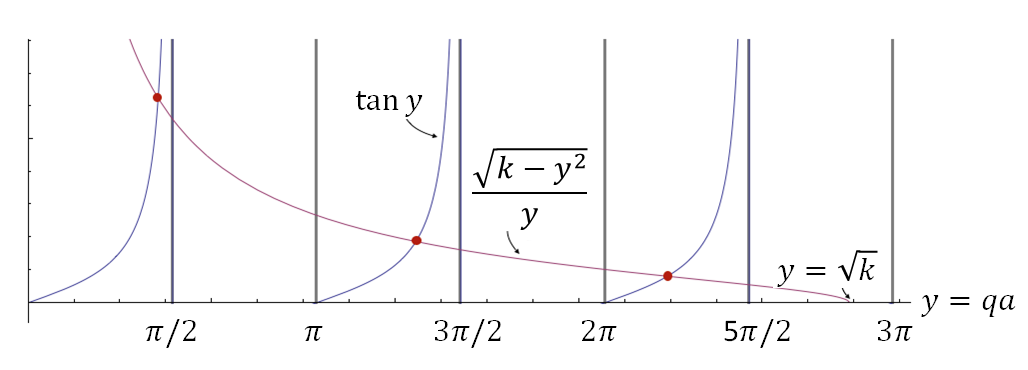
\includegraphics[width=\textwidth]{immagini/cap_10/fig_10_3.png}
\end{figure}
\\
Si noti come il numero di intersezioni cresce al crescere di $k$, ossia \textbf{esistono tanti più stati legati quanto più la buca di potenziale è profonda}.\\
inoltre esiste sempre almeno una intersezione (ed in particolare una sola per $k<\pi$), ossia \textbf{esiste sempre almeno uno stato legato per la particella}.\\
Consideriamo ora le \textbf{autofunzioni dispari}, della forma:
\begin{equation}
\begin{cases}
\psi (x) = A'e^{\lambda x} \quad x<-a;\\
\psi (x) = B'\sin(qx) \quad -a<x<a;\\
\psi (x) = -A'e^{\lambda x} \quad x>a.\end{cases} 
\end{equation}
In questo caso le condizioni di continuità della f.d.o. e della sua derivata nel punto $x=-a$ si scrivono:
\begin{equation}
\begin{cases}
A'e^{-\lambda a} =-B'\sin(qa) ;\\
A' \lambda e^{-\lambda a} = B'q \cos (qa);\end{cases} 
\end{equation}
e forniscono la condizione:
\begin{equation}
q \cot (qa) =- \lambda.
\label{eq:cap10_2}
\end{equation}
Espressa in termini di $y$ e $k$ questa equazione si scrive:
\begin{equation}
\frac{\sqrt{k-y^2}}{y}= -\cot (y) \qquad \qquad (y^2 \leq k),
\end{equation}
e le soluzioni si ottengono graficamente dalle intersezioni qui rappresentate:
\newpage
\begin{figure}[!htbp]
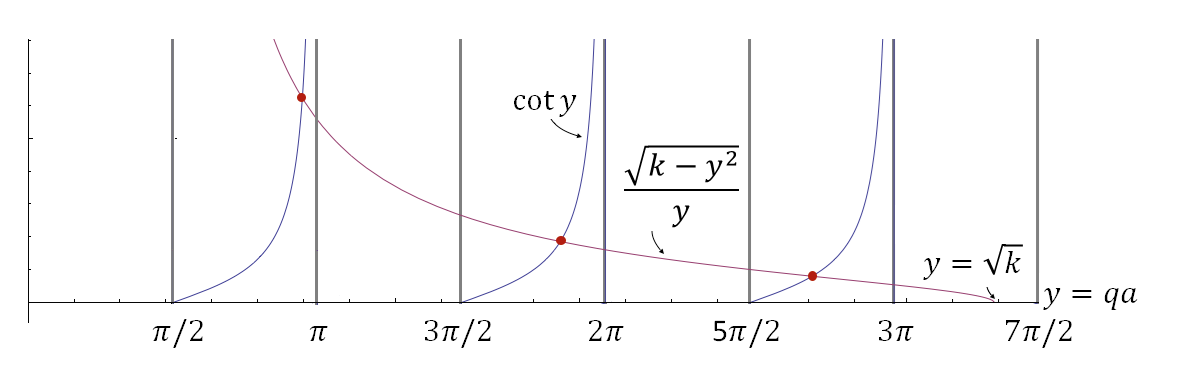
\includegraphics[width=\textwidth]{immagini/cap_10/fig_10_4.png}
\end{figure}
\[ \textrm{N.B. } \tan (y+\pi/2) = -\cot (y) \]\\
Si noti come, anche in questo caso, il numero di intersezioni cresce al crescere di $k$, ossia \textbf{il numero di stati legati cresce al crescere della profondità della buca}.\\
Tuttavia l'eq. (\ref{eq:cap10_2}) \textbf{ammette soluzioni solo se} $\mathbf{k\geq \pi^2/4}$,\textbf{ ossia}:
\begin{equation}
\frac{2mV_0 a^2}{\hbar ^2} \geq \frac{\pi ^2}{4}.
\end{equation}
Se questa condizione non è soddisfatta, esiste solo uno stato legato corrispondente ad un'autofunzione pari.
\section{Gradino di potenziale}
Consideriamo un \textbf{campo di forze in cui il potenziale presenta una discontinuità}, della forma:\\
\begin{minipage}{.55\textwidth}
\begin{equation}
V(x)=
\begin{cases}
0 \quad \textrm{ per } x<0;\\
V_0 \quad \textrm{per } x<0.
\end{cases}
\end{equation}
\end{minipage}
\hspace{.2cm}
\begin{minipage}{.4\textwidth}
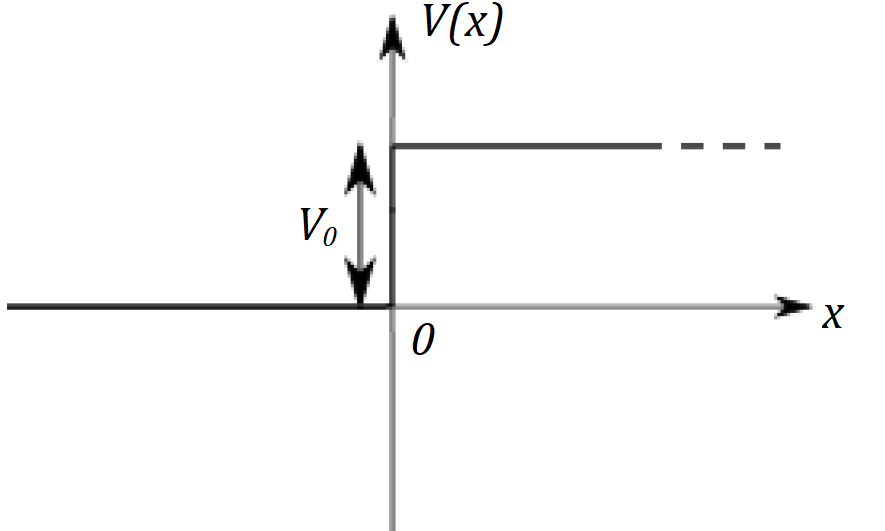
\includegraphics[width=5cm]{immagini/cap_10/fig_10_5.png}
\end{minipage}\\
Secondo la \textbf{meccanica classica}, una particella con energia $E>V_0$, che si muove in un tale campo da sinistra verso destra, arrivata alla barriera di potenziale continua a muoversi nella stessa direzione ma con velocità minore. Se invece la sua energia è $E<V_0$, arrivata alla barriera la particella si riflette da essa e riprende il moto in direzione opposta.\\
Nella \textbf{meccanica quantistica} compare un fenomeno nuovo: anche per $E>V_0$ la particella può essere riflessa dalla barriera di potenziale. Ricaviamo tale risultato.\\
L'equazione di Schr\"{o}dinger in presenza del potenziale è:
\begin{equation}
-\frac{\hbar ^2}{2m}\frac{d^2 \psi}{dx^2}+ V(x)\psi= E\psi, 
\end{equation}
ossia:
\begin{equation}
-\frac{\hbar ^2}{2m}\frac{d^2 \psi}{dx^2}= -\frac{2m}{\hbar ^2}\left( E-V(x)\right) \psi. 
\end{equation}
Considerando il caso $\mathbf{E>V_0}$ e ponendo:
\begin{equation}
k^2=\frac{2mE}{\hbar ^2} \qquad q^2=\frac{2m\left( E- V_0\right)}{\hbar ^2},
\end{equation}
otteniamo per l'equazione di Schr\"{o}dinger nelle due regioni $x<0$ ed $x>0$ la forma:
\begin{equation}
\begin{cases}
\displaystyle{\frac{d^2 \psi}{dx^2}= -k^2 \psi \quad x<0,}\\
\\
\displaystyle{\frac{d^2 \psi}{dx^2}= -q^2 \psi \quad x>0.}\\
\end{cases}
\end{equation}
Se assumiamo che la particella incidente giunga da sinistra verso destra possiamo scrivere la soluzione dell'equazione di Schr\"{o}dinger nella forma:
\begin{eqnarray}
&\psi(x)& = Ae^{ikx}+Be^{-ikx} \quad x<0,\nonumber\\
\\
&\psi(x)& = Ce^{iqx} \qquad \ \quad \qquad x>0.\nonumber
\end{eqnarray}
Ovviamente nella regione $x>0$ non esiste un'onda di ritorno. Le componenti $\displaystyle{Be^{-ikx}}$ e $\displaystyle{Ce^{iqx}}$ rappresentano invece l'\textbf{onda riflessa} e l'\textbf{onda trasmessa} dal gradino di potenziale.\\
La f.d.o. deve essere continua in tutto lo spazio, ed in particolare dunque nel punto $x=0$. Inoltre, malgrado la discontinuità del potenziale nel punto $x=0$, possiamo dimostrare che anche la derivata prima della f.d.o. deve essere continua in questo punto. Si ha infatti:
\begin{eqnarray}
& &\lim _{\varepsilon \rightarrow 0 } \left[ \left( \frac{\partial \psi}{\partial x}\right) _{\varepsilon}-\left( \frac{\partial \psi}{\partial x}\right)_{-\varepsilon}\right]=\lim _{\varepsilon \rightarrow 0 } \int_{-\varepsilon} ^{\varepsilon} dx\ \frac{d}{dx} \left( \frac{d\psi}{dx}\right)= \nonumber \\
& & = \lim _{\varepsilon \rightarrow 0 } -\frac{2m}{\hbar ^2}\int_{-\varepsilon} ^{\varepsilon} dx\ \frac{d}{dx} \left(E-V(x) \right)\psi=0,
\end{eqnarray}
dove l'ultima uguaglianza segue dal fatto che l'integrale di una funzione finita tende a zero nel limite in cui la larghezza dell'intervallo di integrazione tende a zero.\\
Imponendo la continuità della f.d.o. e della sua derivata prima nel punto $x=0$ si ottiene:
\begin{equation}
\begin{cases}
A+B=C \quad \qquad \quad \textrm{ continuità di }\psi\textrm{ in }x=0,\\
k\left(A-B \right) =qC\qquad \textrm{ continuità di }\psi '\textrm{ in }x=0.
\end{cases}
\end{equation}
Da queste due condizioni risultano determinate due costanti, $B$ e $C$, mentre la terza, $A$, dipende dalla normalizzazione della f.d.o. ossia dal flusso incidente.\\
Moltiplicando la prima equazione per q e sottraendo da questa la seconda si ottiene:
\begin{equation}
\left( q-k \right) A + \left( q+k \right)B=0,
\end{equation}
da cui:
\begin{equation}
B= \frac{k-q}{k+q}A.
\label{eq:cap10_3}
\end{equation}
Similmente, moltiplicando la prima equazione per k e sommando a questa la seconda equazione si ottiene:
\begin{equation}
2kA=\left( k+q \right)C,
\end{equation}
ossia:
\begin{equation}
C=\frac{2k}{k+q}A.
\label{eq:cap10_4}
\end{equation}
Le equazioni (\ref{eq:cap10_3}) e (\ref{eq:cap10_4}) risolvono completamente il problema posto.\\
Definiamo il \textbf{coefficiente di riflessione $R$} come il rapporto tra le densità di corrente dell'onda riflessa ($\displaystyle{Be^{-ikx}}$) e la densità di corrente dell'onda incidente ($\displaystyle{Ae^{ikx}}$):
\begin{equation}
R=\frac{|j_r|}{j_i}.
\end{equation}
Analogamente si definisce il \textbf{coefficiente di trasmissione $T$} come il rapporto tra la densità di corrente trasmessa ($\displaystyle{Ce^{iqx}}$) e la densità di corrente dell'onda incidente ($\displaystyle{Ae^{ikx}}$):
\begin{equation}
T=\frac{j_t}{j_i}.
\end{equation}
\textbf{I coefficienti di riflessione e di trasmissione rappresentano allora le probabilità che la particella incidente sul gradino di potenziale venga rispettivamente riflessa oppure trasmessa}.\\
Per una generica onda piana della forma:
\begin{equation}
\psi= Ae^{ikx},
\end{equation}
la densità di corrente è data da:
\begin{equation}
j=\frac{\hbar}{m}\Im \left(\psi ^* \frac{d\psi}{dx} \right)= |A|^2\frac{\hbar k}{m}.
\end{equation}
I coefficienti di riflessione e trasmissione risultano allora:
\begin{eqnarray}
R=\frac{|j_r|}{j_i}= \frac{|B|^2}{|A|^2}=\left(\frac{k-q}{k+q}\right)^2;\nonumber \\
\\
T=\frac{j_t}{j_i}= \frac{|C|^2 q}{|A|^2 k}=\left(\frac{4kq}{k+q}\right)^2.\nonumber 
\end{eqnarray}
Un valore di $R$ differente da zero indica una corrispondente probabilità non nulla che la particella venga riflessa dal gradino di potenziale in completo contrasto con le previsioni classiche. Tuttavia, in accordo con l'intuizione, nel limite in cui l'energia della particella è molto maggiore dell'altezza del gradino, $E\gg V_0$ ossia $k\simeq q$ la probabilità di riflessione tende a zero:
\begin{equation}
R\simeq 0\quad  \textrm{ per } E\gg V_0.
\end{equation}
Osserviamo che ovviamente è verificata la relazione:
\begin{equation}
R+T=1,
\label{eq:cap10_5}
\end{equation}
in accordo con l'interpretazione probabilistica dei coefficienti di riflessione e trasmissione.\\
L'eq. (\ref{eq:cap10_5}) può essere usata come conseguenza generale dell'equazione di continuità:
\begin{equation}
\frac{\partial \left(\psi^* \psi \right)}{\partial t}+ \frac{\partial j}{\partial x}=0,
\end{equation}
che esprime appunto la conservazione della probabilità. Poiché infatti non vi è alcuna dipendenza dal tempo nel problema, questa equazione implica che $j(x)$ è indipendente da $x$. Quindi il flusso in $x<0$ deve essere uguale al flusso in $x>0$. Si ha:
\begin{eqnarray}
j\left( x<0 \right) &=& \frac{\hbar}{m} \Im \left. \left( \psi ^* \frac{\partial \psi}{\partial x} \right) \right| _{x<0} = \nonumber \\
&=& \frac{\hbar}{m} \Im \left[ \left( A^* e^{-ikx} + B^* e^{ikx}\right)ik \left( A e^{ikx} + B e^{-ikx}\right)\right]= \nonumber \\
&=&\frac{\hbar k}{m} \Im \left[ i\left( |A|^2 - |B|^2 +AB^* e^{2ikx}- A^* B e^{-2ikx}\right)\right]= \nonumber \\
&=&\frac{\hbar k}{m} \Im \left[ i\left( |A|^2 - |B|^2 +2i \Im \left( A B^* e^{2ikx}\right) \right)\right]= \nonumber \\
&=& \frac{\hbar k}{m}\left( |A|^2 - |B|^2\right)= j_i- |j_r|,
\end{eqnarray}
e
\begin{equation}
j\left( x>0 \right) = |C| \frac{\hbar q}{m}= j_t,
\end{equation}
pertanto vale la condizione
\begin{equation}
j_i = |j_r|+ j_t,
\end{equation}
che equivale all'eq. (\ref{eq:cap10_5}) per i coefficienti di riflessione e trasmissione.\\
Un \textbf{fenomeno puramente quantistico} si osserva quando il potenziale $V_0$ è negativo ed in modulo molto grande:\\
\begin{minipage}{.7\textwidth}
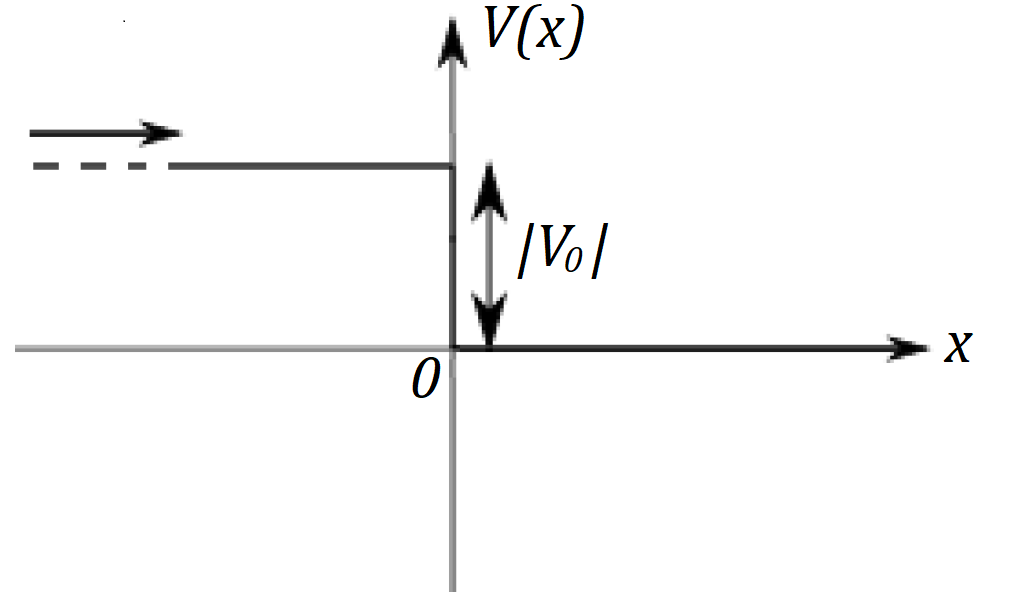
\includegraphics[width=.9\textwidth]{immagini/cap_10/fig_10_6.png}
\end{minipage}
\hspace{.5cm}
\begin{minipage}{.1\textwidth}
\[V_0<0\]
\[|V_0| \gg E\]
\end{minipage}\\ \\
Classicamente la particella proveniente da sinistra verso destra, giunta al salto di potenziale, prosegue nella sua direzione con maggiore velocità.\\
La previsione della meccanica quantistica è invece la seguente: poiché
\begin{equation}
q^2=\frac{2m}{\hbar ^2}\left( E+ |V_0| \right) \gg \frac{2mE}{\hbar ^2} = k^2,
\end{equation}
Si trova:
\begin{equation}
R=\left( \frac{q-k}{q+k} \right) ^2 \simeq 1, \qquad T=\frac{4qk}{\left( q+k \right) ^2} \simeq 0,
\end{equation}
ossia la \textbf{particella viene riflessa} con probabilità quasi uno.\\
Un altro caso che interessa considerare è quello in cui la particella incide sul gradino di potenziale con energia minore dell'altezza del gradino:\\
\begin{minipage}{.7\textwidth}
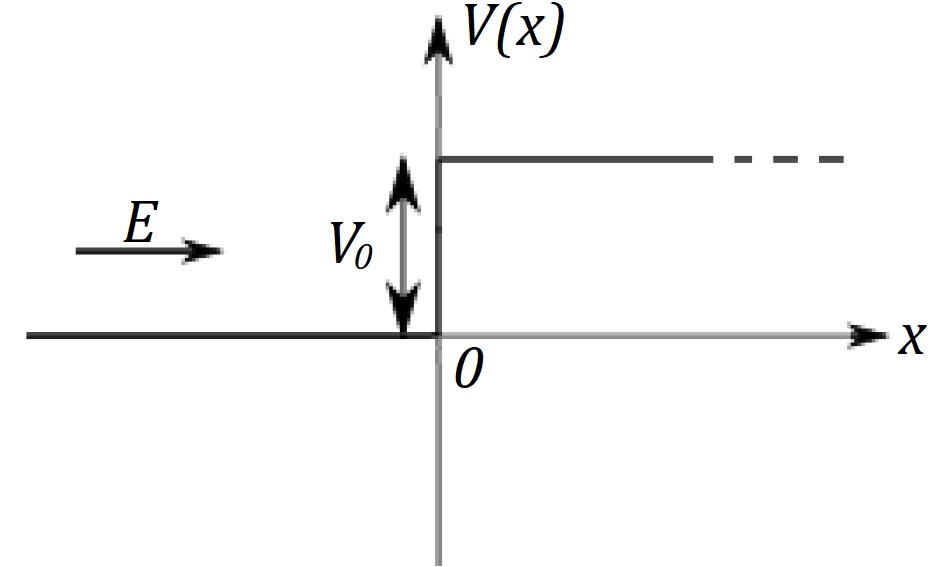
\includegraphics[width=.9\textwidth]{immagini/cap_10/fig_10_7.png}
\end{minipage}
\hspace{.5cm}
\begin{minipage}{.1\textwidth}
\[E<V_0\]
\end{minipage}\\ \\

In questo caso:
\begin{equation}
q^2=\frac{2m}{\hbar ^2}\left( E- V_0 \right)<0,
\end{equation}
ossia $q$ è immaginario. La soluzione dell'equazione di Schr\"{o}dinger, nella regione $x<0$, è della forma:
\begin{equation}
\psi (x) = Ce^{-|q|x} \qquad \qquad x<0
\end{equation}
(giacché la soluzione $\displaystyle{Ce^{+|q|x}}$ diverge all'infinito).\\
Tutti i risultati ottenuti precedentemente si modificano allora per la sostituzione:
\begin{equation}
q \rightarrow i|q|
\end{equation}
e quindi, in particolare, per i coefficienti $B$ e $C$ si ha:
\begin{equation}
B=\frac{k-i|q|}{k+i|q|}A, \qquad C=\frac{2k}{k+i|q|}.
\end{equation}
il coefficiente di riflessione $R$ risulta allora:
\begin{equation}
R=\frac{|B|^2}{|A|^2}=\frac{k-i|q|}{k+i|q|}\frac{k+i|q|}{k+i|q|}=1,
\end{equation}
mentre il coefficiente di trasmissione è nullo,
\begin{equation}
T=0,
\end{equation}
essendo sempre nulla la densità di corrente associata ad una f.d.o. reale.\\
Pertanto, come in meccanica classica, si ha in questo caso \textbf{riflessione totale}. Ciò nonostante osserviamo che la \textbf{f.d.o. non si annulla nella regione classicamente proibita} e vi è dunque una probabilità non nulla di osservare la particella in questa regione. Come vedremo in seguito, questo fenomeno puramente quantistico di penetrazione in una regione classicamente proibita consente il cosiddetto \textbf{effetto tunnel}, ossia l'attraversamento di una barriera di potenziale che bloccherebbe completamente la particella secondo la descrizione classica.
\section{Barriera di potenziale -  effetto tunnel}
Consideriamo un campo di forze il cui potenziale ha l'andamento\\
\begin{minipage}{.55\textwidth}
\begin{equation}
V(x)=
\begin{cases}
0 \qquad x<-a,\\
V_0 \quad -a<x<a,\\
0 \qquad x>-a.
\end{cases}
\end{equation}
\end{minipage}
\hspace{.2cm}
\begin{minipage}{.4\textwidth}
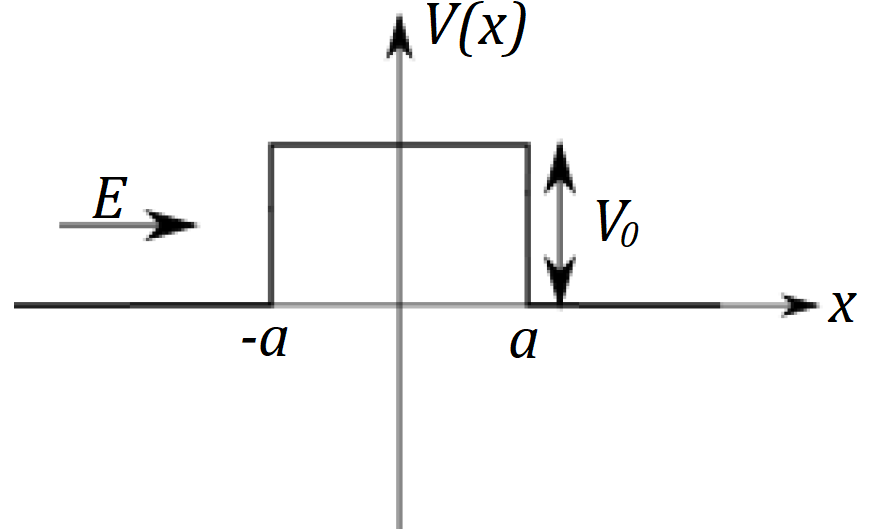
\includegraphics[width=5cm]{immagini/cap_10/fig_10_8.png}
\end{minipage}\\

Studiamo il moto della particella che giunge da sinistra con energia $\mathbf{E<V_0}$. Classicamente la particella, giunta alla barriera, viene riflessa e torna indietro.\\
Consideriamo invece la descrizione quantistica. \textbf{L'equazione di Schr\"{o}dinger} è
\begin{equation}
\begin{cases}
\displaystyle{-\frac{\hbar ^2}{2m}\frac{d^2 \psi}{d x^2}=E \psi \qquad \qquad x <-a \ \textrm{ e }\  x>a,}\\
\\
\displaystyle{-\frac{\hbar ^2}{2m}\frac{d^2 \psi}{d x^2}+V_0 \psi=E \psi \qquad -a  \leq x \leq a.}
\end{cases}
\end{equation}
Ponendo:
\begin{equation}
k^2= \frac{2mE}{\hbar ^2} \qquad \qquad \lambda ^2= \frac{2m}{\hbar ^2} \left( V_0 - E \right),
\end{equation}
dove $k$ e $\lambda $ sono parametri reali, possiamo scrivere l'equazione di Schr\"{o}dinger nella forma:
\begin{equation}
\begin{cases}
\displaystyle{\frac{d^2 \psi}{d x^2}= -k ^2 \psi \qquad  x <-a \ \textrm{ e }\  x>a,}\\
\\
\displaystyle{\frac{d^2 \psi}{d x^2}= \lambda ^2 \psi \qquad 	\ -a  < x < a.}
\end{cases}
\end{equation}
Le \textbf{soluzioni} di queste equazioni differenziali con la condizione al contorno che in assenza di barriera lo stato è rappresentato da un'onda piana che si propaga nella direzione delle $x$ positive sono:
\begin{equation}
\begin{cases}
\displaystyle{\psi (x) = e^{ikx}+Ae^{-ikx} \qquad \ x <-a,}\\
\\
\displaystyle{\psi (x) = Be^{\lambda x}+Ce^{-\lambda x} \qquad  -a< x <a,}\\
\\
\displaystyle{\psi (x) = De^{ikx} \qquad \qquad \qquad \ x >a.}
\end{cases}
\end{equation}
La \textbf{normalizzazione} scelta corrisponde ad aver fissato a
\begin{equation}
j_i= \frac{\hbar k}{m}
\end{equation}
il flusso dell'onda incidente.\\
imponendo la \textbf{continuità della f.d.o. e della sua derivata prima} nei punti $x=\pm a$ si ottiene il seguente sistema di equazioni:
\begin{equation}
\begin{cases}
\displaystyle{e^{-ika}+ Ae^{ika}= Be^{-\lambda a} + C e^{\lambda a}}\\
\\
\displaystyle{ik \left(e^{-ika}+ Ae^{ika}\right)= \lambda \left(Be^{-\lambda a} - C e^{\lambda a}\right)}\\
\\
\displaystyle{Be^{\lambda a} + Ce^{-\lambda a}= De^{ika}}\\
\\
\displaystyle{\lambda \left(Be^{\lambda a} -Ce^{-\lambda a} \right)= ikDe^{ika}}
\end{cases}
\end{equation}
Moltiplichiamo la prima equazione per $ik$ e sommiamo e sottraiamo la seconda equazione.\\
Eseguiamo le stesse operazioni sulla terza e sulla quarta equazione. Si ottiene in tal modo:
\begin{equation}
\begin{cases}
\displaystyle{2ike^{-ika}= B \left(ik+\lambda\right)e^{-\lambda a} +C \left(ik-\lambda\right)e^{\lambda a} }\\
\\
\displaystyle{2ikAe^{ika}= B \left(ik-\lambda\right)e^{-\lambda a} +C \left(ik+\lambda\right)e^{\lambda a} }\\
\\
\displaystyle{B\left(ik+\lambda\right)e^{\lambda a} + C\left(ik-\lambda\right)e^{-\lambda a} = 2ikD e^{ika}}\\
\\
\displaystyle{B\left(ik-\lambda\right)e^{\lambda a} + C\left(ik+\lambda\right)e^{-\lambda a} =0}
\end{cases}
\label{eq:cap10_10}
\end{equation}
La prima e la quarta di queste equazioni costituiscono un sistema di due equazioni nelle due incognite $B$ e $C$. Moltiplicando la prima equazione per $(ik+\lambda) e^{-\lambda a }$ e la quarta per $(ik-\lambda) e^{\lambda a }$ e sottraendo poi la quarta dalla prima si ottiene
\begin{equation}
B\left[ (ik+\lambda)^2 e^{-2\lambda a }-(ik-\lambda)^2 e^{2\lambda a }\right]= 2ik(ik+\lambda) e^{-\left(ik+\lambda\right) a },
\end{equation} 
da cui
\begin{equation}
B\left[ (-k^2+\lambda ^2+2ik\lambda) e^{-2\lambda a }-(-k^2+\lambda-2ik\lambda) e^{2\lambda a }\right]= 2ik(ik+\lambda) e^{-\left(ik+\lambda\right) a },
\end{equation}
e infine
\begin{equation}
B=\frac{ik\left(ik+\lambda \right)e^{-\left(ik+\lambda\right) a }}{\left(k^2-\lambda^2\right)\sinh \left(2\lambda a\right)+2ik\lambda \cosh\left(2\lambda a\right)}.
\end{equation}
Il coefficiente $C$ si ottiene da $B$ scambiando $\lambda \rightarrow -\lambda$:
\begin{equation}
C=\frac{-ik\left(ik-\lambda \right)e^{-\left(ik-\lambda\right) a }}{\left(k^2-\lambda^2\right)\sinh \left(2\lambda a\right)+2ik\lambda \cosh\left(2\lambda a\right)}.
\end{equation}
I coefficienti $A$ e $D$ si ottengono infine sostituendo questi risultati nella seconda e terza equazione del sistema. Si trova
\begin{eqnarray}
& 2ikAe^{ika}= B \left(ik-\lambda\right)e^{-\lambda a} +C \left(ik+\lambda\right)e^{\lambda a}=&\nonumber \\
\nonumber\\
& = \displaystyle{\frac{ik\left(-k^2-\lambda ^2 \right)e^{-2\lambda a }e^{-ika }-ik\left(-k^2-\lambda ^2 \right)e^{2\lambda a }e^{-ika }}{\left(k^2-\lambda^2\right)\sinh \left(2\lambda a\right)+2ik\lambda \cosh\left(2\lambda a\right)}=} &\nonumber \\
\nonumber \\
&\displaystyle{ =\frac{2ik\left(k^2+\lambda ^2 \right)\sinh\left(2\lambda a\right)e^{-ika}}{\left(k^2-\lambda^2\right)\sinh \left(2\lambda a\right)+2ik\lambda \cosh\left(2\lambda a\right)}},&
\end{eqnarray}
e
\begin{eqnarray}
&2ikD e^{ika} = B\left(ik+\lambda\right)e^{\lambda a} + C\left(ik-\lambda\right)e^{-\lambda a} = &\nonumber \\
\nonumber\\
& = \displaystyle{\frac{ik\left(-k^2 + \lambda ^2 +2ik\lambda\right)e^{-ika}-ik\left(-k^2 + \lambda ^2 -2ik\lambda\right)e^{-ika}}{\left(k^2-\lambda^2\right)\sinh \left(2\lambda a\right)+2ik\lambda \cosh\left(2\lambda a\right)}=} &\nonumber \\
\nonumber \\
&\displaystyle{ =\frac{-4k^2\lambda e^{-ika}}{\left(k^2-\lambda^2\right)\sinh \left(2\lambda a\right)+2ik\lambda \cosh\left(2\lambda a\right)}},&
\end{eqnarray}
ossia:
\begin{equation}
A=\frac{\left(k^2+\lambda ^2\right)\sinh\left(2\lambda a \right)e^{-2ika}}{\left(k^2-\lambda^2\right)\sinh \left(2\lambda a\right)+2ik\lambda \cosh\left(2\lambda a\right)},
\end{equation}
e
\begin{equation}
D=\frac{2ik\lambda e^{-2ika}}{\left(k^2-\lambda^2\right)\sinh \left(2\lambda a\right)+2ik\lambda \cosh\left(2\lambda a\right)}.
\end{equation}
La quantità che ci interessa calcolare è il \textbf{coefficiente di trasmissione}
\begin{equation}
T=\frac{j_t}{j_i}=|D|^2,
\end{equation}
che risulta dunque valere
\begin{equation}
T=\frac{4k^2 \lambda ^2}{\left(k^2-\lambda^2\right) ^2\sinh ^2\left(2\lambda a\right)+4k^2\lambda ^2\cosh ^2\left(2\lambda a\right)},
\end{equation}
ossia
\begin{equation}
T=\frac{4k^2 \lambda ^2}{\left(k^2+\lambda^2\right) ^2\sinh ^2\left(2\lambda a\right)+4k^2\lambda ^2}.
\end{equation}
Il risultato per questo coefficiente (diverso da zero) implica che \textbf{vi è una probabilità non nulla che la particella attraversi la barriera di potenziale}. Questo fenomeno, puramente quantistico, è noto con il nome di \textbf{effetto tunnel}.\\
Frequentemente risulta soddisfatta la condizione
\begin{equation}
2\lambda a \gg 1.
\end{equation}
Poiché
\begin{equation}
\frac{1}{\lambda}=\frac{\hbar}{\sqrt{2m\left(V_0 - E \right)}}=\frac{\hbar}{\sqrt{2mE\left(V_0/E - 1 \right)}}=\frac{\hbar /p}{\sqrt{\left(V_0/E - 1 \right)}},
\end{equation}
questa condizione equivale a
\begin{equation}
2a \gg \frac{\hbar /p}{\sqrt{\left(V_0/E - 1 \right)}},
\end{equation}
ossia la larghezza della barriera risulta molto maggiore della lunghezza d'onda di De Broglie della particella divisa per il fattore $\sqrt{\left(V_0/E - 1 \right)}$ (tipicamente di $O(1)$.\\
In queste condizioni, nell'espressione del coefficiente di trasmissione, possiamo trascurare $e^{-2\lambda a}$ e $1$ rispetto ad $e^{2\lambda a}$ per ottenere
\begin{eqnarray}
T &\overset{\lambda a \gg 1}{\simeq}& \left(\frac{4k\lambda}{k^2+\lambda ^2} \right) ^2 e^{-4\lambda a} =\left(\frac{4\lambda /k}{1+\lambda ^2/k^2} \right) ^2 e^{-4\lambda a}= \nonumber \\
\nonumber \\
&=&16\frac{\left(V_0 /E-1\right)}{\left(V_0 /E \right) ^2}e^{-4a\sqrt{\frac{2m}{\hbar ^2}\left(V_0-E\right)}},
\end{eqnarray}
ossia
\begin{equation}
T \simeq 16 \left(\frac{E}{V_0} \right) \left(1-\frac{E}{V_0}\right) e^{-4a\sqrt{\frac{2m}{\hbar ^2}\left(V_0-E\right)}}.
\end{equation}
Questa espressione mostra come la probabilità di trasmissione della particella attraverso la barriera di potenziale decresce esponenzialmente con la lunghezza della barriera ($2a$) e quanto più l'altezza della barriera ($V_0$) eccede l'energia della particella ($E$).\\
Le stesse conclusioni continuano a valere in condizioni più generali. Utilizzando la cosidetta \textbf{approssimazione WKB\footnote{WKB: Wentzel, Kramers, Brillouin}o approssimazione quasi-classica}, è possibile infatti derivare per il coefficiente di trasmissione l'espressione:
\begin{equation}
T \approx e^{-2 \int_{barr.} dx\ \sqrt{\frac{2m}{\hbar ^2}\left[ V(x)-E \right]}},
\end{equation}
valida per potenziali $V(x)$ non troppo rapidamente variabili nello spazio.\\
Gli esempi di effetto tunnel sono abbastanza comuni nella fisica atomica e nucleare. Discutiamo qui di seguito due esempi brevemente.
\subsection{Emissione fredda}
L'emissione fredda è un fenomeno che consiste nell' \textbf{emissione di elettroni da parte della superficie di un metallo quando all'esterno della superficie viene applicato un campo elettrico $E$}.\\
Il fenomeno può essere spiegato nel modo seguente. Gli elettroni in un metallo sono confinati all'interno da un potenziale che in prima approssimazione può essere descritto da una buca di profondità finita:

Nello stato fondamentale del metallo tutti i livelli di energia di singolo elettrone sono riempiti fino all'energia di Fermi. La differenza tra l'energia di Fermi e la cima della buca rappresenta l'energia necessaria per estrarre un elettrone dal metallo, ossia la \textbf{funzione lavoro} $w$.\\
Gli elettroni possono essere estratti dal metallo trasferendogli energia, o mediante fotoni o per riscaldamento.\\
Tuttavia \textbf{è} anche \textbf{possibile estrarre elettroni dal metallo senza fornire a questi alcuna energia} ma applicando un campo elettrico $\mathscr{E}$ all'esterno del metallo.\\
In questo caso infatti, il potenziale visto da un elettrone che si trova al livello di fermi cambia, per effetto del campo esterno, da $w+\varepsilon _F$ a $w+\varepsilon _F-e\mathscr{E}x$:
\[w+\varepsilon _F-e\mathscr{E}a=\varepsilon _F\]
\[a= w/(e\mathscr{E})\]
L'elettrone può allore essere emesso per \textbf{effetto tunnel}.\\
la probabilità di emissione è:
\begin{equation}
T \approx \exp \left[-2 \int_{0} ^{a} dx\ \sqrt{\frac{2m}{\hbar ^2} (\underbrace{w+\varepsilon _F-e\mathscr{E}x}_{V(x)}-\underbrace{\varepsilon _F}_{E}})\right].
\end{equation}
Calcoliamo l'integrale:
\begin{equation}
\int _{0} ^{a} \left( w-e\mathscr{E}x \right) ^{1/2}= \left. -\frac{1}{e\mathscr{E}}\left( w-e\mathscr{E}x \right) ^{3/2}\frac{2}{3}\right| _0 ^a =\frac{2}{3}\frac{w^{3/2}}{e\mathscr{E}}.
\end{equation}
Pertanto:
\begin{equation}
T \approx \exp \left[-\frac{4}{3}\left(\frac{2m}{\hbar ^2}\right)^{1/2}\frac{w^{3/2}}{e\mathscr{E}}\right].
\end{equation}
\subsection{Decadimento $\alpha$}
L'esperienza mostra che gli elementi di numero atomico $Z>81$ sono radioattivi, ossia decadono emettendo particelle $\alpha$ (nuclei di elio) o $\beta$ (elettroni) e trasformandosi così in altri elementi.\\
Indichiamo qui un \textbf{semplice modello per descrivere i decadimenti} $\mathbf{\alpha}$ le cui previsioni risultano in buon accordo con le osservazioni sperimentali.\\
In questo modello il decadimento del nucleo in una particella $\alpha$ ed un nucleo ``prodotto'' è descritto come l'emissione, per effetto tunnel, della particella $\alpha$ attraverso una barriera di potenziale causata dall'interazione coulombiana tra il nucleo prodotto e la particella $\alpha$:
\[\frac{Z_1 Z_2 e^2}{b}=E\]
Il raggio $R$ definisce le dimensioni del nucleo. Per $r<R$ la particella risente  del potenziale all'interno del nucleo, schematizzato da una buca. Per $r>R$ il potenziale è coulombiano: $V(r)=Z_1 Z_2 e^2/r$ dove $Z_1$ è la carica del nucleo prodotto e $Z_2=2$ la carica della particella $\alpha$.\\
Affinché il decadimento $\alpha$ (per effetto tunnel) possa avere luogo, la particella $\alpha$ all'interno del nucleo in questo modello deve avere energia $E$ positiva, ossia non deve trovarsi in uno stato legato.\\
La \textbf{probabilità di emissione} della particella $\alpha$ per effetto tunnel è:
\begin{equation}
T \approx \exp \left[ -2 \int _R ^b dr\ \sqrt{\frac{2m}{\hbar ^2}\left(\frac{Z_1 Z_2 e^2}{r}-E\right)}\right].
\end{equation}
Calcoliamo l'integrale:
\begin{eqnarray}
&\displaystyle{\int _R ^b dr\ \left(\frac{Z_1 Z_2 e^2}{r}-E\right)^{1/2}=\left(Z_1 Z_2 e^2\right)^{1/2}\int _R ^b \frac{dr}{\sqrt{r}}\left(1-\frac{Er}{Z_1 Z_2 e^2}\right)=}& \nonumber \\
&\displaystyle{=\left(Z_1 Z_2 e^2\right)^{1/2}\int _R ^b \frac{dr}{\sqrt{r}}\left(1-\frac{r}{b}\right)\overset{s=r/b}{=}}&\nonumber \\
&=\displaystyle{\left(Z_1 Z_2 e^2 b\right)^{1/2}\int _{R/b} ^1 ds\ s^{-1/2} (1-s)^{1/2}}.&
\end{eqnarray}
La piccolezza del raggio nucleare fa sì che risulta sempre valida con buona approssimazione la condizione
\begin{equation}
R\ll b \quad \Rightarrow \quad E \ll \frac{Z_1 Z_2 e^2}{r}
\end{equation}
Risulta pertanto possibile sostituire nel precedente integrale l'estremo inferiore di integrazione, $R/b$, con $0$. L'integrale si riduce quindi ad una costante adimensionale il cui valore,
\begin{equation}
\int _{0} ^1 ds\ s^{-1/2} (1-s)^{1/2}= \frac{\pi}{2},
\end{equation}
si può ottenere effettuando il cambio di variabile $s= \sin^2 \alpha$ (ma non è comunque rilevante per quanto segue).\\
Si trova pertanto:
\begin{eqnarray}
T&\approx & \exp \left[ -\frac{\pi}{(\hbar ^2 /2m)^{1/2}}\left(Z_1 Z_2 e^2 b\right)^{1/2}\right]= \nonumber \\
&=&\exp \left[ -\frac{\pi}{(\hbar ^2 /2m)^{1/2}}\frac{e^2}{\sqrt{E}}\right],
\end{eqnarray}
ossia
\begin{equation}
T \approx e^{-C\frac{Z_1}{\sqrt{E}}},
\end{equation}
che evidenzia la dipendenza della probabilità di decadimento dal numero atomico $Z_1$ del nucleo che decade e dall'energia $E=mv^2/2$ della particella $\alpha$ prodotta nel decadimento.\\
La probabilità di decadimento $\alpha$ del nucleo, T, è inversamente proporzionale alla \textbf{vita media} $\mathbf{\tau}$ del nucleo:
\begin{equation}
\tau=\frac{C'}{T}=e^{C'\frac{Z_1}{\sqrt{E}}},
\end{equation}
o, equivalentemente,
\begin{equation}
\log \tau = \log C' + \frac{C Z_1}{\sqrt{E}}.
\end{equation}
Questo andamento risulta ben confermato dalle misure sperimentali.
\section{Risoluzione dell'eq. di Schr\"{o}dinger per la barriera di potenziale in termini di f.d.o. simmetriche e anti-simmetriche}
L'equazione di Schr\"{o}dinger per la barrirea di potenziale può anche essere risolta, in modo conveniente, in termini di autofunzioni pari e dispari:
\begin{equation}
\psi _S (x) =
\begin{cases}
\displaystyle{e^{ikx} + A_s e^{-ikx} \qquad x<-a,}\\
B_S \cosh (\lambda x) \quad -a<x<a,\\
\displaystyle{e^{-ikx} + A_S e^{ikx} \qquad x>a.}
\end{cases}
\end{equation}
\begin{equation}
\psi _A (x) =
\begin{cases}
\displaystyle{e^{ikx} + A_A e^{-ikx} \qquad x<-a,}\\
B_A \sinh (\lambda x) \quad -a<x<a,\\
\displaystyle{-e^{-ikx} - A_A e^{ikx} \qquad x>a.}
\end{cases}
\end{equation}
Successivamente, una volta determinate le costanti $A$ e $B$ mediante le condizioni di continuità sulle f.d.o. e sulle derivate prime, si costruisce l'opportuna combinazione lineare per il problema dato:
\begin{equation}
\psi (x) =\frac{1}{2}\left(\psi _S (x) + \psi _A (x) \right) =
\begin{cases}
\displaystyle{e^{ikx} + \frac{1}{2}\left(A_S+A_A\right) e^{-ikx}} \\
\\
\displaystyle{\frac{1}{2}B_S \cosh (\lambda x )+ \frac{1}{2} B_A \sinh (\lambda x)} \\
\\
\displaystyle{\frac{1}{2}\left(A_S - A_A \right) e^{ikx}}
\end{cases}
\end{equation}
Vediamo, in particolare, che $\displaystyle{D=\frac{1}{2}\left( A_s - A_A \right)}$.\\
Calcoliamo il coefficiente $D$ utilizzando questo metodo.\\
Le condizioni di continuità per la f.d.o. simmetrica e per la sua derivata prima nel punto $x=a$ si scrivono
\begin{equation}
\begin{cases}
\displaystyle{B_S \cosh (\lambda a) = e^{-ika}+ A_S e^{ika}}\\
\displaystyle{\lambda B_S \sinh (\lambda a) = -ik e^{-ika}+ ikA_S e^{ika}}
\end{cases}
\label{eq:cap10_6}
\end{equation}
Per la simmetria della f.d.o. queste condizioni garantiscono anche la continuità della f.d.o. e della sua derivata nel punto $x=-a$.\\
Il sistema di equazioni (\ref{eq:cap10_6}) può essere facilmente risolto per $A_S$ moltiplicando la prima equazione per $\lambda \sinh (\lambda a)$, la seconda per $\cosh (\lambda a)$ e sottraendo l'una dall'altra:
\begin{equation}
\left(\lambda \sinh (\lambda a)+ ik\cosh (\lambda a) \right)e^{-ika}+ A_S \left(\lambda \sinh (\lambda a)-ik \cosh (\lambda a) \right)e^{ika}=0,
\end{equation}
da cui
\begin{equation}
A_S=-\frac{\lambda \sinh (\lambda a)+ik \cosh (\lambda a)}{\lambda \sinh (\lambda a)-ik \cosh (\lambda a)}e^{-2ika}.
\label{eq:cap10_7}
\end{equation}
La determinazione del coefficiente $A_A$ della f.d.o antisimmetrica procede in modo analogo. in questo caso le condizioni di continuità della f.d.o. e della sua derivata conducono al sistema
\begin{equation}
\begin{cases}
\displaystyle{B_A \sinh (\lambda a) = e^{-ika}- A_A e^{ika}}\\
\displaystyle{\lambda B_A \cosh (\lambda a) = ik e^{-ika}- ikA_A e^{ika}}
\end{cases}
\label{eq:cap10_8}
\end{equation}
Questo sistema differisce dal sistema (\ref{eq:cap10_6}) per lo scambio\\ $\sinh (\lambda a) \leftrightarrow -\cosh (\lambda a)$. Possiamo quindi scrivere direttamente dall'eq. (\ref{eq:cap10_7}) la soluzione per il coefficiente $A_A$:
\begin{equation}
A_A=-\frac{\lambda \cosh (\lambda a)+ik \sinh (\lambda a)}{\lambda \cosh (\lambda a)-ik \sinh (\lambda a)}e^{-2ika}.
\label{eq:cap10_9}
\end{equation}
dalle eq. (\ref{eq:cap10_7}) e (\ref{eq:cap10_9}) ricaviamo infine l'espressione cercata per il coefficiente $D$:
\begin{eqnarray}
D&=&\frac{1}{2}\left( A_S - A_A \right)= \nonumber \\
&=& -\frac{1}{2}e^{-2ika}\bigl[ \left( \lambda \sinh (\lambda a)+ ik \cosh (\lambda a )\right)\cdot\left( \lambda \cosh (\lambda a)- ik \sinh (\lambda a )\right)\nonumber \\ &-& \left( \lambda \cosh (\lambda a)+ ik \sinh (\lambda a )\right)\cdot \left( \lambda \sinh (\lambda a)- ik \cosh (\lambda a )\right)\bigr]/\bigl[ (\lambda \sinh (\lambda a)\nonumber\\
&-& ik\cosh (\lambda a ) \cdot (\lambda \cosh (\lambda a ) - ik \sinh (\lambda a ) \bigr]= \nonumber \\
&=& -\frac{1}{2}e^{-2ika} \frac{-2ik\lambda \sinh ^2 (\lambda a) + 2ik \lambda \cosh ^2 (\lambda a)}{ \left(\lambda ^2 - k^2 \right) \sinh (\lambda a ) \cosh (\lambda a) - ik\lambda \left(\sinh ^2 (\lambda a) + \cosh ^2 (\lambda a ) \right)}.\nonumber \\
\end{eqnarray}
Utilizzando le relazioni:
\begin{eqnarray}
& &\cosh ^2 x - \sinh ^2 x=1 \nonumber \\
& &\cosh ^2 x + \sinh ^2 x=\cosh 2x  \\
& &2 \cosh  x \sinh  x=\sinh 2x \nonumber 
\end{eqnarray}
possiamo riscrivere il coefficiente $D$ nella forma
\begin{equation}
D=\frac{2ik\lambda e^{-2ika}}{\left(k^2-\lambda^2\right)\sinh \left(2\lambda a\right)+2ik\lambda \cosh\left(2\lambda a\right)},
\end{equation}
che coincide con il risultato precedentemente ottenuto.
\section{Risoluzione dell'eq. di Schr\"{o}dinger per la barriera di potenziale nel limite $\mathbf{\lambda a \ll 1}$}
Consideriamo il sistema di equazioni (\ref{eq:cap10_10})e risolviamolo nel limite $\lambda a \ll 1$:
\begin{equation}
\begin{cases}
\displaystyle{2ik\ e^{-ika}=B\left( ik+\lambda\right)e^{-\lambda a} + C\left( ik-\lambda\right)e^{\lambda a}}\\
\\
\displaystyle{2ikA e^{ika}=B\left( ik-\lambda\right)e^{-\lambda a} + C\left( ik+\lambda\right)e^{\lambda a}}\\
\\
\displaystyle{B\left( ik+\lambda\right)e^{\lambda a} + C\left( ik-\lambda\right)e^{-\lambda a}}= 2ikD e^{ika}\\
\\
\displaystyle{B\left( ik-\lambda\right)e^{\lambda a} + C\left( ik+\lambda\right)e^{-\lambda a}}= 0\\
\end{cases}
\end{equation} 
dalla quarta equazione ricaviamo:
\begin{equation}
B=-\frac{(ik+\lambda)}{(ik-\lambda)}e^{-2 \lambda a } C,
\end{equation}
ossia $B$ è esponenzialmente piccolo rispetto a $C$.  nella prima equazione possiamo quindi trascurare il termine proporzionale a $Be^{-\lambda a}$ rispetto a quello proporzionale a $Ce^{\lambda a }$. Si ottiene in tal modo:
\begin{equation}
C= \frac{2ik}{(ik-\lambda)}e^{-ika}e^{-\lambda a},
\end{equation}
e dunque, combinando con la precedente equazione, anche
\begin{equation}
B=-\frac{2ik(ik+\lambda)}{(ik-\lambda)^2}e^{-ik a }e^{-3 \lambda a }.
\end{equation}
Possiamo ora ricavare il coefficiente $D$ utilizzando la terza delle equazioni del sistema. \\
In questa equazione i termini $Be^{\lambda a }$ e $Ce^{-\lambda a }$ sono dello stesso ordine di grandezza (entrambi proporzionali a $e^{-2\lambda a}$). Si ottiene dunque
\begin{eqnarray}
2ikDe^{-ika}&=& 2ike^{-ika}e^{-2\lambda a} \left[-\frac{(ik+\lambda)^2}{(ik-\lambda)^2}+1\right]= \nonumber \\
&=& 2ike^{-ika}e^{-2\lambda a}\frac{(ik-\lambda)^2-(ik+\lambda)^2}{(ik-\lambda)^2}= \nonumber \\
&=& 2ike^{-ika}e^{-2\lambda a}\left( -\frac{4ik\lambda}{(ik-\lambda)^2}\right),
\end{eqnarray}
da cui
\begin{equation}
D= -\frac{4ik\lambda}{(ik-\lambda)^2}e^{-2ika}e^{-2\lambda a}.
\end{equation}
il coefficiente di trasmissione risulta allora
\begin{equation}
T=|D|^2= \left(\frac{4k\lambda}{k^2+\lambda^2}\right) ^2 e^{-4\lambda a},
\end{equation}
in accordo con quanto ottenuto precedentemente nel limite $\lambda a \ll 1$.\\
Osserviamo infine che dalla seconda equazione del sistema, trascurando il termine $Be^{-\lambda a}$ (di $O(e^{-4\lambda a})$ ) rispetto al termine $Ce^{\lambda a}$ (di $O(1)$) si ottiene
\begin{equation}
A=\frac{(ik+\lambda)}{(ik-\lambda)}e^{-ika}\qquad \Rightarrow \qquad R=|A|^2=1+O(e^{-4\lambda a}).
\end{equation}
\end{document}